% Options for packages loaded elsewhere
\PassOptionsToPackage{unicode}{hyperref}
\PassOptionsToPackage{hyphens}{url}
%
\documentclass[
]{article}
\usepackage{amsmath,amssymb}
\usepackage{lmodern}
\usepackage{iftex}
\ifPDFTeX
  \usepackage[T1]{fontenc}
  \usepackage[utf8]{inputenc}
  \usepackage{textcomp} % provide euro and other symbols
\else % if luatex or xetex
  \usepackage{unicode-math}
  \defaultfontfeatures{Scale=MatchLowercase}
  \defaultfontfeatures[\rmfamily]{Ligatures=TeX,Scale=1}
\fi
% Use upquote if available, for straight quotes in verbatim environments
\IfFileExists{upquote.sty}{\usepackage{upquote}}{}
\IfFileExists{microtype.sty}{% use microtype if available
  \usepackage[]{microtype}
  \UseMicrotypeSet[protrusion]{basicmath} % disable protrusion for tt fonts
}{}
\makeatletter
\@ifundefined{KOMAClassName}{% if non-KOMA class
  \IfFileExists{parskip.sty}{%
    \usepackage{parskip}
  }{% else
    \setlength{\parindent}{0pt}
    \setlength{\parskip}{6pt plus 2pt minus 1pt}}
}{% if KOMA class
  \KOMAoptions{parskip=half}}
\makeatother
\usepackage{xcolor}
\usepackage[margin=1in]{geometry}
\usepackage{color}
\usepackage{fancyvrb}
\newcommand{\VerbBar}{|}
\newcommand{\VERB}{\Verb[commandchars=\\\{\}]}
\DefineVerbatimEnvironment{Highlighting}{Verbatim}{commandchars=\\\{\}}
% Add ',fontsize=\small' for more characters per line
\usepackage{framed}
\definecolor{shadecolor}{RGB}{248,248,248}
\newenvironment{Shaded}{\begin{snugshade}}{\end{snugshade}}
\newcommand{\AlertTok}[1]{\textcolor[rgb]{0.94,0.16,0.16}{#1}}
\newcommand{\AnnotationTok}[1]{\textcolor[rgb]{0.56,0.35,0.01}{\textbf{\textit{#1}}}}
\newcommand{\AttributeTok}[1]{\textcolor[rgb]{0.77,0.63,0.00}{#1}}
\newcommand{\BaseNTok}[1]{\textcolor[rgb]{0.00,0.00,0.81}{#1}}
\newcommand{\BuiltInTok}[1]{#1}
\newcommand{\CharTok}[1]{\textcolor[rgb]{0.31,0.60,0.02}{#1}}
\newcommand{\CommentTok}[1]{\textcolor[rgb]{0.56,0.35,0.01}{\textit{#1}}}
\newcommand{\CommentVarTok}[1]{\textcolor[rgb]{0.56,0.35,0.01}{\textbf{\textit{#1}}}}
\newcommand{\ConstantTok}[1]{\textcolor[rgb]{0.00,0.00,0.00}{#1}}
\newcommand{\ControlFlowTok}[1]{\textcolor[rgb]{0.13,0.29,0.53}{\textbf{#1}}}
\newcommand{\DataTypeTok}[1]{\textcolor[rgb]{0.13,0.29,0.53}{#1}}
\newcommand{\DecValTok}[1]{\textcolor[rgb]{0.00,0.00,0.81}{#1}}
\newcommand{\DocumentationTok}[1]{\textcolor[rgb]{0.56,0.35,0.01}{\textbf{\textit{#1}}}}
\newcommand{\ErrorTok}[1]{\textcolor[rgb]{0.64,0.00,0.00}{\textbf{#1}}}
\newcommand{\ExtensionTok}[1]{#1}
\newcommand{\FloatTok}[1]{\textcolor[rgb]{0.00,0.00,0.81}{#1}}
\newcommand{\FunctionTok}[1]{\textcolor[rgb]{0.00,0.00,0.00}{#1}}
\newcommand{\ImportTok}[1]{#1}
\newcommand{\InformationTok}[1]{\textcolor[rgb]{0.56,0.35,0.01}{\textbf{\textit{#1}}}}
\newcommand{\KeywordTok}[1]{\textcolor[rgb]{0.13,0.29,0.53}{\textbf{#1}}}
\newcommand{\NormalTok}[1]{#1}
\newcommand{\OperatorTok}[1]{\textcolor[rgb]{0.81,0.36,0.00}{\textbf{#1}}}
\newcommand{\OtherTok}[1]{\textcolor[rgb]{0.56,0.35,0.01}{#1}}
\newcommand{\PreprocessorTok}[1]{\textcolor[rgb]{0.56,0.35,0.01}{\textit{#1}}}
\newcommand{\RegionMarkerTok}[1]{#1}
\newcommand{\SpecialCharTok}[1]{\textcolor[rgb]{0.00,0.00,0.00}{#1}}
\newcommand{\SpecialStringTok}[1]{\textcolor[rgb]{0.31,0.60,0.02}{#1}}
\newcommand{\StringTok}[1]{\textcolor[rgb]{0.31,0.60,0.02}{#1}}
\newcommand{\VariableTok}[1]{\textcolor[rgb]{0.00,0.00,0.00}{#1}}
\newcommand{\VerbatimStringTok}[1]{\textcolor[rgb]{0.31,0.60,0.02}{#1}}
\newcommand{\WarningTok}[1]{\textcolor[rgb]{0.56,0.35,0.01}{\textbf{\textit{#1}}}}
\usepackage{graphicx}
\makeatletter
\def\maxwidth{\ifdim\Gin@nat@width>\linewidth\linewidth\else\Gin@nat@width\fi}
\def\maxheight{\ifdim\Gin@nat@height>\textheight\textheight\else\Gin@nat@height\fi}
\makeatother
% Scale images if necessary, so that they will not overflow the page
% margins by default, and it is still possible to overwrite the defaults
% using explicit options in \includegraphics[width, height, ...]{}
\setkeys{Gin}{width=\maxwidth,height=\maxheight,keepaspectratio}
% Set default figure placement to htbp
\makeatletter
\def\fps@figure{htbp}
\makeatother
\setlength{\emergencystretch}{3em} % prevent overfull lines
\providecommand{\tightlist}{%
  \setlength{\itemsep}{0pt}\setlength{\parskip}{0pt}}
\setcounter{secnumdepth}{-\maxdimen} % remove section numbering
\usepackage{booktabs}
\usepackage{longtable}
\usepackage{array}
\usepackage{multirow}
\usepackage{wrapfig}
\usepackage{float}
\usepackage{colortbl}
\usepackage{pdflscape}
\usepackage{tabu}
\usepackage{threeparttable}
\usepackage{threeparttablex}
\usepackage[normalem]{ulem}
\usepackage{makecell}
\usepackage{xcolor}
\ifLuaTeX
  \usepackage{selnolig}  % disable illegal ligatures
\fi
\IfFileExists{bookmark.sty}{\usepackage{bookmark}}{\usepackage{hyperref}}
\IfFileExists{xurl.sty}{\usepackage{xurl}}{} % add URL line breaks if available
\urlstyle{same} % disable monospaced font for URLs
\hypersetup{
  pdftitle={Assignment 5},
  pdfauthor={Mia Guarnieri, Lauren Harris, Wade Sedgwick},
  hidelinks,
  pdfcreator={LaTeX via pandoc}}

\title{Assignment 5}
\author{Mia Guarnieri, Lauren Harris, Wade Sedgwick}
\date{2023-05-08}

\begin{document}
\maketitle

\hypertarget{source-the-function}{%
\subsection{Source the function}\label{source-the-function}}

\begin{Shaded}
\begin{Highlighting}[]
\FunctionTok{source}\NormalTok{(}\FunctionTok{here}\NormalTok{(}\StringTok{"R"}\NormalTok{, }\StringTok{"Catm.r"}\NormalTok{))}
\end{Highlighting}
\end{Shaded}

\hypertarget{create-the-random-sample-using-lhs}{%
\subsection{Create the random sample using
lhs}\label{create-the-random-sample-using-lhs}}

\begin{Shaded}
\begin{Highlighting}[]
\CommentTok{\# set the seed so it is random}
\FunctionTok{set.seed}\NormalTok{(}\DecValTok{1}\NormalTok{)}

\CommentTok{\# designate parameters}
\NormalTok{pnames }\OtherTok{=} \FunctionTok{c}\NormalTok{(}\StringTok{"height"}\NormalTok{, }\StringTok{"k\_d"}\NormalTok{, }\StringTok{"k\_o"}\NormalTok{, }\StringTok{"v"}\NormalTok{)}

\CommentTok{\# how many parameters}
\NormalTok{npar }\OtherTok{=}  \FunctionTok{length}\NormalTok{(pnames)}

\CommentTok{\# how many samples}
\NormalTok{nsample }\OtherTok{=} \DecValTok{100}

\CommentTok{\# generate samples using lhs function}
\NormalTok{parm\_quant }\OtherTok{=} \FunctionTok{randomLHS}\NormalTok{(nsample, npar)}

\CommentTok{\# rename columns to match variables}
\FunctionTok{colnames}\NormalTok{(parm\_quant) }\OtherTok{=}\NormalTok{ pnames }

\CommentTok{\# creating parameter dataframe}
\NormalTok{parm }\OtherTok{=} \FunctionTok{as.data.frame}\NormalTok{(}\FunctionTok{matrix}\NormalTok{(}\AttributeTok{nrow=}\FunctionTok{nrow}\NormalTok{(parm\_quant), }\AttributeTok{ncol=}\FunctionTok{ncol}\NormalTok{(parm\_quant)))}
\FunctionTok{colnames}\NormalTok{(parm) }\OtherTok{=}\NormalTok{ pnames}

\CommentTok{\# generating sample distributions for our parameters}
\NormalTok{parm[,}\StringTok{"height"}\NormalTok{] }\OtherTok{=} \FunctionTok{qunif}\NormalTok{(parm\_quant[,}\StringTok{"height"}\NormalTok{], }\AttributeTok{min =} \FloatTok{9.5}\NormalTok{, }\AttributeTok{max =} \FloatTok{10.5}\NormalTok{)}
\NormalTok{parm[,}\StringTok{"v"}\NormalTok{] }\OtherTok{=} \FunctionTok{qnorm}\NormalTok{(parm\_quant[,}\StringTok{"v"}\NormalTok{], }\AttributeTok{mean =} \DecValTok{250}\NormalTok{, }\AttributeTok{sd =} \DecValTok{30}\NormalTok{)}
\NormalTok{parm[,}\StringTok{"k\_d"}\NormalTok{] }\OtherTok{=} \FunctionTok{qnorm}\NormalTok{(parm\_quant[,}\StringTok{"k\_d"}\NormalTok{], }\AttributeTok{mean =} \FloatTok{0.7}\NormalTok{, }\AttributeTok{sd =} \FloatTok{0.01}\NormalTok{)}
\NormalTok{parm[,}\StringTok{"k\_o"}\NormalTok{] }\OtherTok{=} \FunctionTok{qnorm}\NormalTok{(parm\_quant[,}\StringTok{"k\_o"}\NormalTok{], }\AttributeTok{mean =} \FloatTok{0.1}\NormalTok{, }\AttributeTok{sd =} \FloatTok{0.01}\NormalTok{)}
\end{Highlighting}
\end{Shaded}

\hypertarget{run-model-for-parameter-sets}{%
\subsection{Run model for parameter
sets}\label{run-model-for-parameter-sets}}

\begin{Shaded}
\begin{Highlighting}[]
\CommentTok{\# run the model}
\NormalTok{cond }\OtherTok{=}\NormalTok{ parm }\SpecialCharTok{\%\textgreater{}\%} \FunctionTok{pmap}\NormalTok{(Catm)}

\CommentTok{\# turn results in to a dataframe for easy display/analysis}
\NormalTok{condsd }\OtherTok{\textless{}{-}} \FunctionTok{as.data.frame}\NormalTok{(}\FunctionTok{unlist}\NormalTok{(cond))}
\FunctionTok{colnames}\NormalTok{(condsd) }\OtherTok{=} \StringTok{"ca"}
\end{Highlighting}
\end{Shaded}

\hypertarget{plot}{%
\subsection{Plot}\label{plot}}

\begin{Shaded}
\begin{Highlighting}[]
\CommentTok{\# add uncertainty bounds on our estimates}
\FunctionTok{ggplot}\NormalTok{(condsd) }\SpecialCharTok{+}
  \FunctionTok{geom\_boxplot}\NormalTok{(}\FunctionTok{aes}\NormalTok{(}\AttributeTok{y =}\NormalTok{ ca)) }\SpecialCharTok{+}
  \FunctionTok{labs}\NormalTok{(}\AttributeTok{y=}\StringTok{"Conductance (mm/s)"}\NormalTok{,}
       \AttributeTok{title =} \StringTok{"Conductance Uncertainty"}\NormalTok{) }\SpecialCharTok{+}
  \FunctionTok{theme}\NormalTok{(}\AttributeTok{axis.text.x =} \FunctionTok{element\_blank}\NormalTok{(),}
        \AttributeTok{axis.ticks.x =} \FunctionTok{element\_blank}\NormalTok{())}
\end{Highlighting}
\end{Shaded}

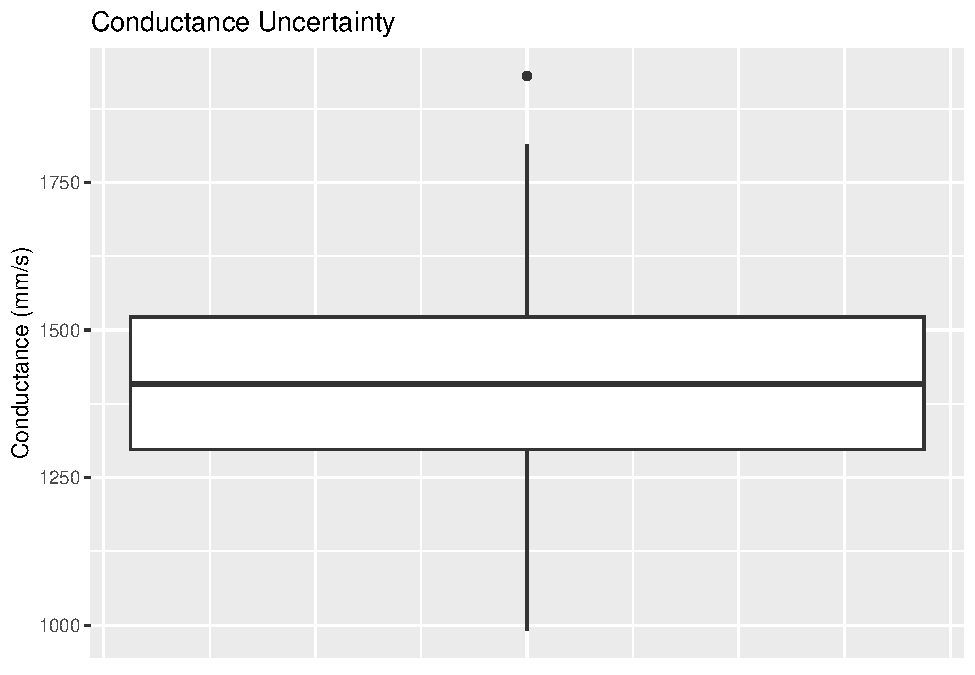
\includegraphics{assignment_4_files/figure-latex/unnamed-chunk-4-1.pdf}

\begin{Shaded}
\begin{Highlighting}[]
\CommentTok{\# cumulative distribution}
\FunctionTok{ggplot}\NormalTok{(condsd, }\FunctionTok{aes}\NormalTok{(}\AttributeTok{y =}\NormalTok{ ca)) }\SpecialCharTok{+}
  \FunctionTok{stat\_ecdf}\NormalTok{() }\SpecialCharTok{+}
  \FunctionTok{labs}\NormalTok{(}\AttributeTok{y =} \StringTok{"Conductance (mm/s)"}\NormalTok{,}
       \AttributeTok{x =} \StringTok{"Empirical Cumulative Distribution Function"}\NormalTok{,}
       \AttributeTok{title =} \StringTok{"Cumulative Conductance Distribution"}\NormalTok{)}
\end{Highlighting}
\end{Shaded}

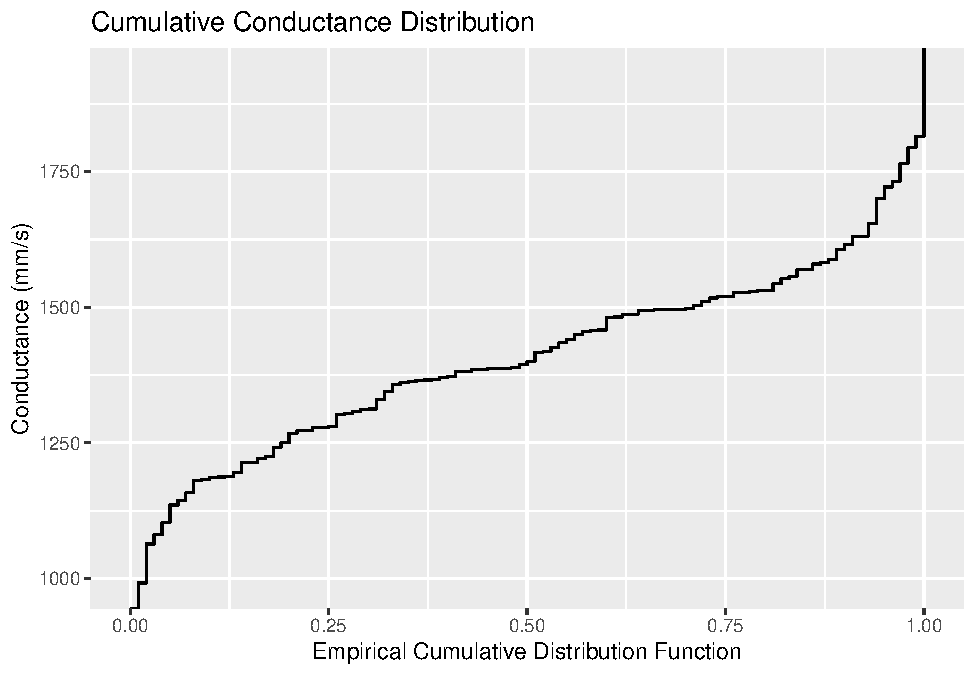
\includegraphics{assignment_4_files/figure-latex/unnamed-chunk-4-2.pdf}

\begin{Shaded}
\begin{Highlighting}[]
\CommentTok{\# plot parameter sensitivity}
\NormalTok{tmp }\OtherTok{=} \FunctionTok{cbind.data.frame}\NormalTok{(condsd, parm)}

\NormalTok{tmp2 }\OtherTok{=}\NormalTok{ tmp }\SpecialCharTok{\%\textgreater{}\%} \FunctionTok{gather}\NormalTok{(}\SpecialCharTok{{-}}\NormalTok{ca, }\AttributeTok{key=}\StringTok{"parm"}\NormalTok{, }\AttributeTok{value=}\StringTok{"parmvalue"}\NormalTok{)}

\FunctionTok{ggplot}\NormalTok{(tmp2, }\FunctionTok{aes}\NormalTok{(parmvalue, ca)) }\SpecialCharTok{+}
  \FunctionTok{geom\_point}\NormalTok{() }\SpecialCharTok{+}
  \FunctionTok{facet\_wrap}\NormalTok{(}\SpecialCharTok{\textasciitilde{}}\NormalTok{ parm, }\AttributeTok{scales=}\StringTok{"free"}\NormalTok{, }\AttributeTok{ncol =} \DecValTok{4}\NormalTok{) }\SpecialCharTok{+}
  \FunctionTok{scale\_x\_continuous}\NormalTok{(}\AttributeTok{n.breaks =} \DecValTok{4}\NormalTok{) }\SpecialCharTok{+}
  \FunctionTok{labs}\NormalTok{(}\AttributeTok{x =} \StringTok{"Parameter"}\NormalTok{,}
       \AttributeTok{y =} \StringTok{"Conductance (mm/s)"}\NormalTok{,}
       \AttributeTok{title =} \StringTok{"Parameter Sensitivity"}\NormalTok{)}
\end{Highlighting}
\end{Shaded}

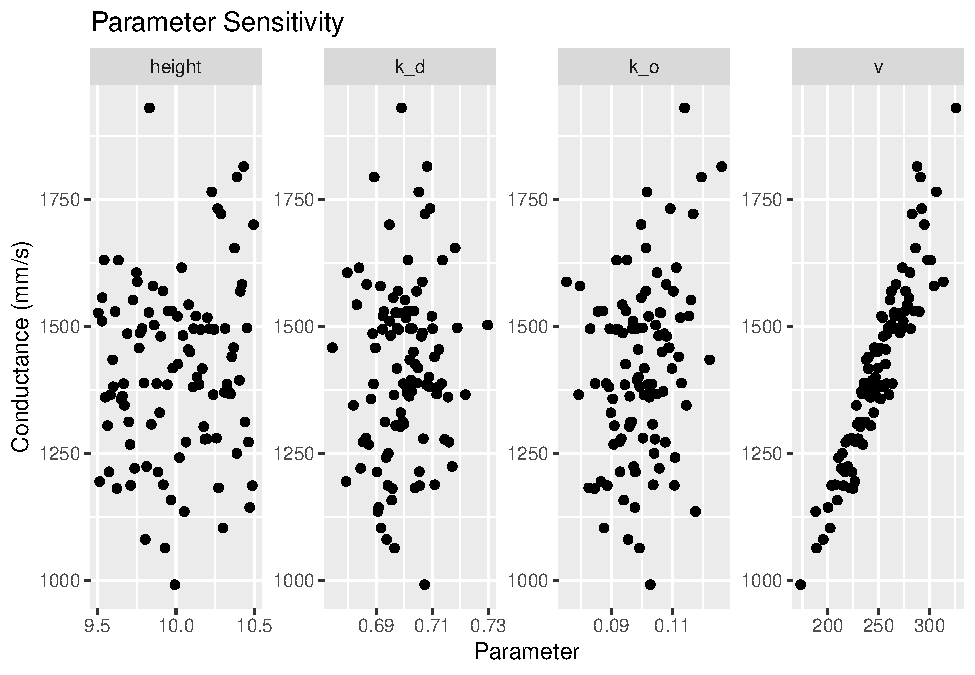
\includegraphics{assignment_4_files/figure-latex/unnamed-chunk-4-3.pdf}

\hypertarget{quantify-sensitivity---pcc}{%
\subsection{Quantify sensitivity -
pcc}\label{quantify-sensitivity---pcc}}

\begin{Shaded}
\begin{Highlighting}[]
\CommentTok{\# calculate and plot partial rank correlation coefficients}
\NormalTok{senresult\_rank }\OtherTok{=} \FunctionTok{pcc}\NormalTok{(parm, condsd}\SpecialCharTok{$}\NormalTok{ca, }\AttributeTok{rank=}\ConstantTok{TRUE}\NormalTok{ )}

\FunctionTok{plot}\NormalTok{(senresult\_rank)}
\end{Highlighting}
\end{Shaded}

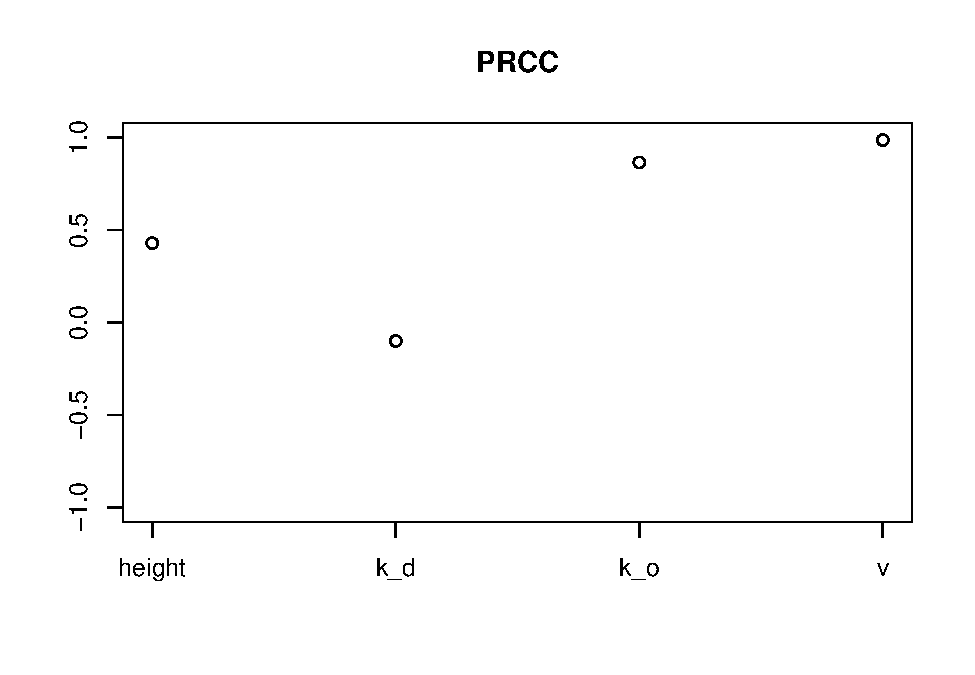
\includegraphics{assignment_4_files/figure-latex/unnamed-chunk-5-1.pdf}

\begin{Shaded}
\begin{Highlighting}[]
\CommentTok{\# extract prcc values from pcc object}

\NormalTok{parm\_prcc }\OtherTok{\textless{}{-}} \FunctionTok{as.data.frame}\NormalTok{(senresult\_rank}\SpecialCharTok{$}\NormalTok{PRCC)}

\FunctionTok{rownames}\NormalTok{(parm\_prcc) }\OtherTok{=} \FunctionTok{c}\NormalTok{(}\StringTok{"Height"}\NormalTok{, }\StringTok{"Zero Plane Displacement (k\_d)"}\NormalTok{, }\StringTok{"Roughness (k\_o)"}\NormalTok{, }\StringTok{"Windspeed (v)"}\NormalTok{)}

\NormalTok{parm\_prcc\_table }\OtherTok{\textless{}{-}}\NormalTok{ parm\_prcc }\SpecialCharTok{\%\textgreater{}\%}
  \FunctionTok{kable}\NormalTok{(}\AttributeTok{digits =} \DecValTok{3}\NormalTok{,}
        \AttributeTok{col.names =} \StringTok{"Partial Rank Correlation Coefficient"}\NormalTok{) }\SpecialCharTok{\%\textgreater{}\%} 
  \FunctionTok{kable\_styling}\NormalTok{(}\AttributeTok{full\_width =} \ConstantTok{FALSE}\NormalTok{) }\SpecialCharTok{\%\textgreater{}\%} 
  \FunctionTok{kable\_paper}\NormalTok{()}

\NormalTok{parm\_prcc\_table}
\end{Highlighting}
\end{Shaded}

\begin{table}
\centering
\begin{tabular}{l|r}
\hline
  & Partial Rank Correlation Coefficient\\
\hline
Height & 0.429\\
\hline
Zero Plane Displacement (k\_d) & -0.100\\
\hline
Roughness (k\_o) & 0.867\\
\hline
Windspeed (v) & 0.988\\
\hline
\end{tabular}
\end{table}

\hypertarget{discussion}{%
\subsection{Discussion}\label{discussion}}

Wind velocity has the highest correlation with atmospheric conductance.
To reduce uncertainty in atmospheric conductance estimates, getting more
accurate and precise wind speeds should be the highest priority. The
height of the vegetation and roughness of terrain also contribute to
atmospheric conductance, but have lower correlation coefficients than
wind velocity, and improving the accuracy of these measurements could
help as well. The zero plane displacement had the lowest correlation
with atmospheric conductance. A higher conductance rate results in more
evaporation and higher water use needs. As climate change gets worse, it
is possible that higher wind speeds will become more frequent and will
lead to higher atmospheric conductance, since conductance is most
sensitive to changes in wind velocity. More variable weather events will
likely lead to more variable conductance, resulting in less certainty in
conductance estimates and water use needs.

\end{document}
